\chapter{Marco teórico}
\pagenumbering{arabic}
\setcounter{page}{10}
\renewcommand{\baselinestretch}{2} %doble espacio paratodo el texto

{\bf Ejemplo:}\par

En este capítulo se presenta una reseña del material bibliográfico investigado con relación a los temas considerados en esta investigación. Los conocimientos investigados son muy amplios, principalmente aquel que ayudó a consolidar las bases del conocimiento científico para elaborar esta tesis, como lo son los temas de optimización combinatoria, complejidad computacional, metaheurísticas, ciencia de la información y logística, conocimientos sin los cuales sería difícil de modelar y solucionar matemática y computacionalmente cualquier tipo de problema de optimización.
\vskip 1cm 

\section{Optimización combinatoria y complejidad computacional}
\subsection{Problemas combinatorios}
\subsection{Heurísticas y metaheurísticas}

\section{Sustentabilidad}

{\bf Ejemplo:}\par

La configuración, característica, jurisdicción administrativa, relaciones económicas, sociales y ambientales de un espacio urbano se define por la población y por la función que ella desarrolla en un área geográfica o región \citep{Bugliarello}. De este modo las ciudades son sistemas dinámicos que interactúan continua y constantemente con su medio ambiente, acompañando las características, perfil, cultura y ritmo de desarrollo económico y social de su población. Los medios de transporte juegan un papel importante en tal ritmo de desarrollo de las ciudades, ya que ellos tienen como función relacional los factores poblacionales con los factores uso del suelo.  
\vskip 1cm
El desarrollo sustentable, (Figura 2.1), estará garantizado si se consideran tres aspectos fundamentales: económico, social y ambiental, donde la intersección de estos aspectos garantiza la calidad de vida en el espacio urbano y el equilibrio en las clases sociales en busca del bienestar \citep{Tanguay}.

\begin{figure}[ht]
\begin{center}
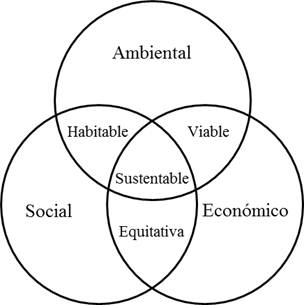
\includegraphics[width=0.3\textwidth]{Figura2}
\end{center}
\begin{center}
\vskip -0.5cm
\caption{\small{Aspectos claves para el desarrollo sustentable.}}
{\small{Fuente: \cite{Tanguay}}}
\end{center}
\end{figure}

\section{Logística directa y reversa}

\subsection{Logística directa}

{\bf Ejemplo:}\par

\cite{Ghiani} entienden que la logística trata de la planificación y control de los flujos de materiales e informaciones relacionadas en las organizaciones, tanto en los sectores público y privado. Además su misión es hacer la entrega de los productos correctos, en el local correcto y en la hora correcta, optimizando los costos operacionales totales del proceso.
satisfaciendo un determinado conjunto de restricciones o condiciones.\par

\subsection{Logística reversa}

{\bf Ejemplo:}\par

En los años 90 se presentaron definiciones generales las cuales vienen siendo mejoradas. \cite{Dekker} presenta una mejora en la definición de logística reversa como  ”el proceso de planificación, implementación y control de los flujos de materias-primas, en procesos de inventarios y bienes acabados, desde el punto de fabricación, distribución o uso, hacia el punto de recuperación o de eliminación”. 
\begin{figure}[ht]
\begin{center}
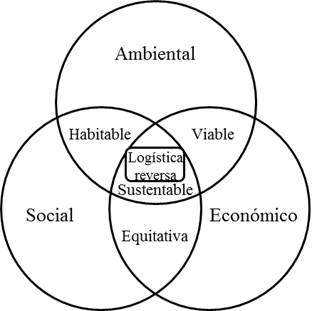
\includegraphics[width=0.3\textwidth]{Figura1}
\end{center}
\begin{center}
\vskip -0.5cm
\caption{\small{Logística reversa incluida en el desarrollo sustentable.}}
{\small{Fuente: Adaptación de \cite{Tanguay}}}
\end{center}
\end{figure}


\subsubsection{Modelos}

\section{Modelamiento y ruteo }

{\bf Ejemplo:}\par

El modelamiento matemático es una alternativa para expresar formalmente hechos reales que pueden ayudar en el proceso de toma de decisiones. El modelamiento permite la simulación de procesos  y de escenarios con la introducción de índices de desempeño que permitan cuantificar los costos y beneficios de la implementación del sistema, la mejoría de la sustentabilidad urbana y por supuesto los índices de contaminación en las grandes ciudades y su impacto en todo el medio ambiente. 

\subsection{Modelos utilizados en los problemas de ruteo de vehículo }

{\bf Ejemplo:}\par

El problema de ruteo de vehículos \citep{Ombuki, Yeun} y sus variantes han ganado mucho interés en la comunidad académica. La intención de estar más cerca a la realidad mediante el modelamiento matemático, hace que se hayan desarrollado nuevos modelos de optimización. \par
\vskip 0.3cm
Según \cite{Sterle} el primer nivel de la red comprende la distribución de la carga desde las plataformas hasta las unidades satélites, utilizando vehículos de carga de mayor tamaño (g).  El segundo nivel, consiste en montar rutas desde las unidades satélites hasta los clientes, usando para este caso vehículos de menor tamaño (v). El modelo de localización y ruteo de vehículos para la distribución de carga propuesto por el autor, además de hacer la conexión de los dos niveles y estudiar su inter relación y dependencia, el modelo busca determinar la cantidad necesaria de plataforma y de unidades satélites considerando el tamaño y dimensionamiento de la flota para el ruteo en dos niveles. 
\vskip 0.2cm
\begin{table}[ht]
\begin{center}
%\vskip -0.5cm
\caption{\small{Resultados computacionales obtenidos en el modelo de \cite{Sterle}}}
\end{center}
\begin{center}
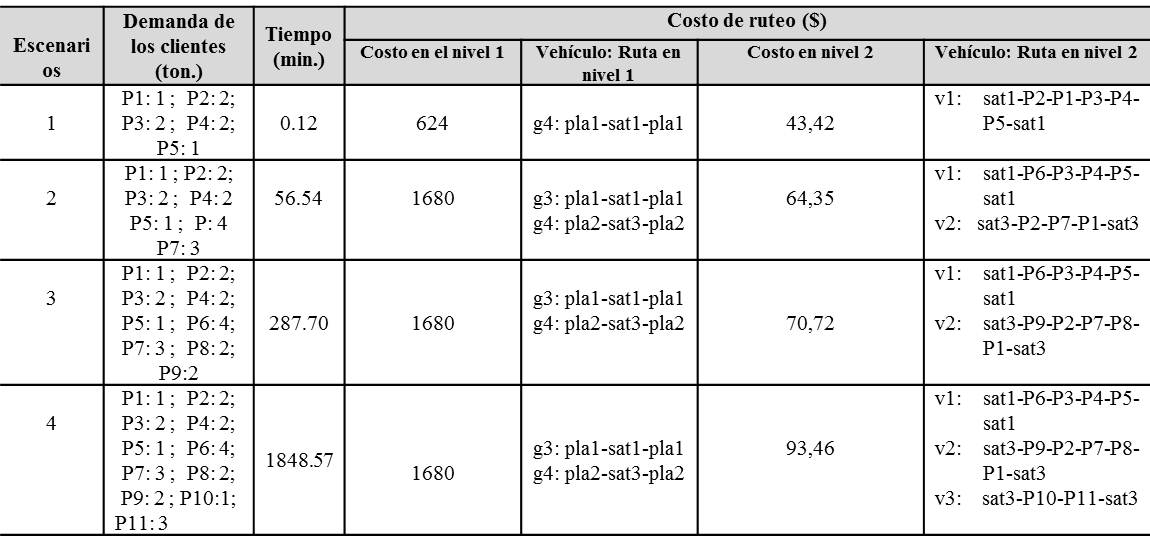
\includegraphics[width=0.7\textwidth]{Tabla1}
\end{center}
\begin{center}
\vskip -0.5cm
{\small{Fuente: Resultados obtenidos con CPLEX.}}
\end{center}
\end{table}